\subsection{Problemstellung}
    Gegeben sei eine Wetterstation mit einem Sensor in einem abgelegenen
    Teil der westlichen Sahara, welche eine Leistungsaufnahme zwischen
    1W bis 2W besitzt. Wie kann eine solche Anlage kostengünstig und
    relativ wartungsfrei betrieben werden?
    \\\\
    Hier lohnt es sich die starke Sonnenenergie der Region
    auszunutzen, eine Solareinrichtung von geringer Größe kann über
    den Tag genug Sonnenenergie sammeln um sowohl die Wetterstation zu
    versorgen als auch eine Batterie zur Überbrückung der Nacht
    aufzuladen.
    \\\\
    Um den dauerhaften Betrieb der Wetterstation gewährleisten zu können
    müssen zu jedem Zeitpunkt 2W an Leistung zur Verfügung stehen.

\subsection{Theorie}
    Eine photovoltaische Zelle wandelt eingehende Leistung \( P_e \)
    mit einem Wirkungsgrad \( \eta \) in ausgehende Leistung \( P_a \)
    um, die eingehende Leistung ist abhängig von der Bestrahlungsstärke,
    also Sonnenlesitung pro Bestrahlungsfläche \( E_e = [\frac{P_s}
    {A_s}] \) und der Fläche \( A \) der photovltaischen Zelle.
        \[ P_a = \eta \cdot P_e \]
    Dabei ist die eingehende Leistung
        \[ P_e = E_e \cdot A\]
    woraus folgt dass
        \[ P_a = \eta \cdot E \cdot A \]
    Von den gegeben Werten kann sowhol der Wirkungsgrad, so wie die
    eingehende Sonnenenergie nur bedingt beeinflusst werden. Damit
    Die benötigte ausgehende Leistung ist also von der Fläche der
    Zelle abhängig.
    \\\\
    Der Wirkungsgrad \( \eta \) einer photovoltaischen Zelle wird zur
    Laborkonditionen getestet, also bei \( T_{STC} = 25 \)°C
    Umgebungstemperatur, \( 1 \mathrm{\frac{kW}{m^2}} \) Bestrahlungs-
    stärke und 1.5 spektraler Distibution \cite{Wiki_SolarEfficiency}.
    \newpage

\subsection{Praxis}
    In der Sahara beträgt die durschnittliche Temperatur am Tag rund
    30°C, die Bestrahlungsstärke rund \( 2 \mathrm{\frac{kW}{m^2}} \)
    bis \( 2.5 \mathrm{\frac{kW}{m^2}} \) und die durschnittliche
    tägliche Sonnenzeit rund 9 Stunden (Sonnenstand höher als 30°)
    \cite{Wiki_SolarAfrica, DateTimeWestSahara}.
    \\\\
    Folgende Werte werden für die nachfolgenden Berechnungen verwendet,
    wovon Basiswirkungsgrad \( \eta_{STC}\) und Temperaturkoeffizenten
    der Leistung \( \gamma \) aus dem Beispieldatenblatt eines
    Solarmoduls entnomment wurden \cite{SolarDatasheet}:
    \begin{itemize}
        \item \( E_e = 2000 \mathrm{\frac{W}{m^2}} \)
        \item \( t_{Tag} = 9 \mathrm{h} \)
        \item \( \eta_{STC} = 0.161 \)
        \item \( \gamma = -\mathrm{\frac{0.0043}{K}} \)
        \item \( T_B = 30 \degree \mathrm{C}\)
    \end{itemize}
    Angesichts der geringen Zeit in der genug Sonnenenergie gesammelt
    werden kann, muss zu dieser Zeit auch die Energie zu Überbrückung der
    restlichen 15 Stunden gesammelt werden. Die gesamte benötigte Energie
    ergibt sich aus:
        \[ E_G = P_G \cdot t_G \]
        \[ E_G = 2 \mathrm{W} \cdot 24 \mathrm{h} = 48 \mathrm{Wh} \]
    Woraus sich wiederum die Tagesleistung \( P_{Tag} \) für die
    Tageszeit \( t_{Tag} \) ergibt:
        \[ P_{Tag}  = \frac{E_G}{t_{Tag}} \]
        \[ P_{Tag} = \frac{48 \mathrm{Wh}}{9 \mathrm{h}} =
        5.\overline{3} \mathrm{W} \]
    Die Temperaturdifferenz und der draus resultierende wirkliche
    Wirkungsgrad bei Betriebstemperatur \( T_B \) ergeben sich aus:
        \[ \Delta T = T_B - T_{STC} \]
        \[ \Delta T = 30 \mathrm{\degree C} - 25 \mathrm{\degree C}
        = 5 \mathrm{K} \]
        \[ \eta = \eta_{STC} + \gamma \Delta T \]
        \[ \eta = 0.161 - \mathrm{\frac{0.0043}{K}} \cdot 5 \mathrm{K}
        = 0.1285 \]
    Daraus folgt die benötigte Größe \( A \) der photovoltaischen
    Zelle in Abhängigkeit von eingehender Sonnenenergie, tatsächlichem
    Wirkungsgrad und benötigter Ausgangsleistung.
        \[ A = \frac{P_a}{\eta E_e} \approx 0.0184464 \mathrm{m^2}
        \approx 185 \mathrm{cm^2} \]
    Bei einer Betriebsspannung von \( U = 24 \mathrm{V} \) wird ein
    maxinmaler Betriebsstrom von \( I_B = 83.\overline{3}
    \mathrm{mA} \) erwartet. Die benötigte Kapazität des Speichermediums
    ergibt sich aus Betriebsstrom und gewünschter Entladungsdauer.
        \[ Q = t_{Nacht} \cdot I_B \]
        \[ Q = 15 \mathrm{h} \cdot 0.08\overline{3} \mathrm{A} =
        1.24\overline{9} \mathrm{Ah} \approx 1250 \mathrm{mAh} \]

\subsection{Konklusion}
    Bei einer photovolatischen Zelle mit einer Fläche von etwa
    \(185 \mathrm{cm^2} \) bis \(200 \mathrm{cm^2} \) ist der
    Energiebadarf einer solchen Wetterstation selbst bei schlechten
    Verhältnissen gedeckt in sofern ein Speichermedium mit einer Kapazität
    von mindestens 1.25Ah zur Verfügung steht. Eine vereinfachte Schaltung
    der Stromversorgung einer solchen Station könnte wie folgt aussehen:
    \begin{figure}[H]
        \centering
        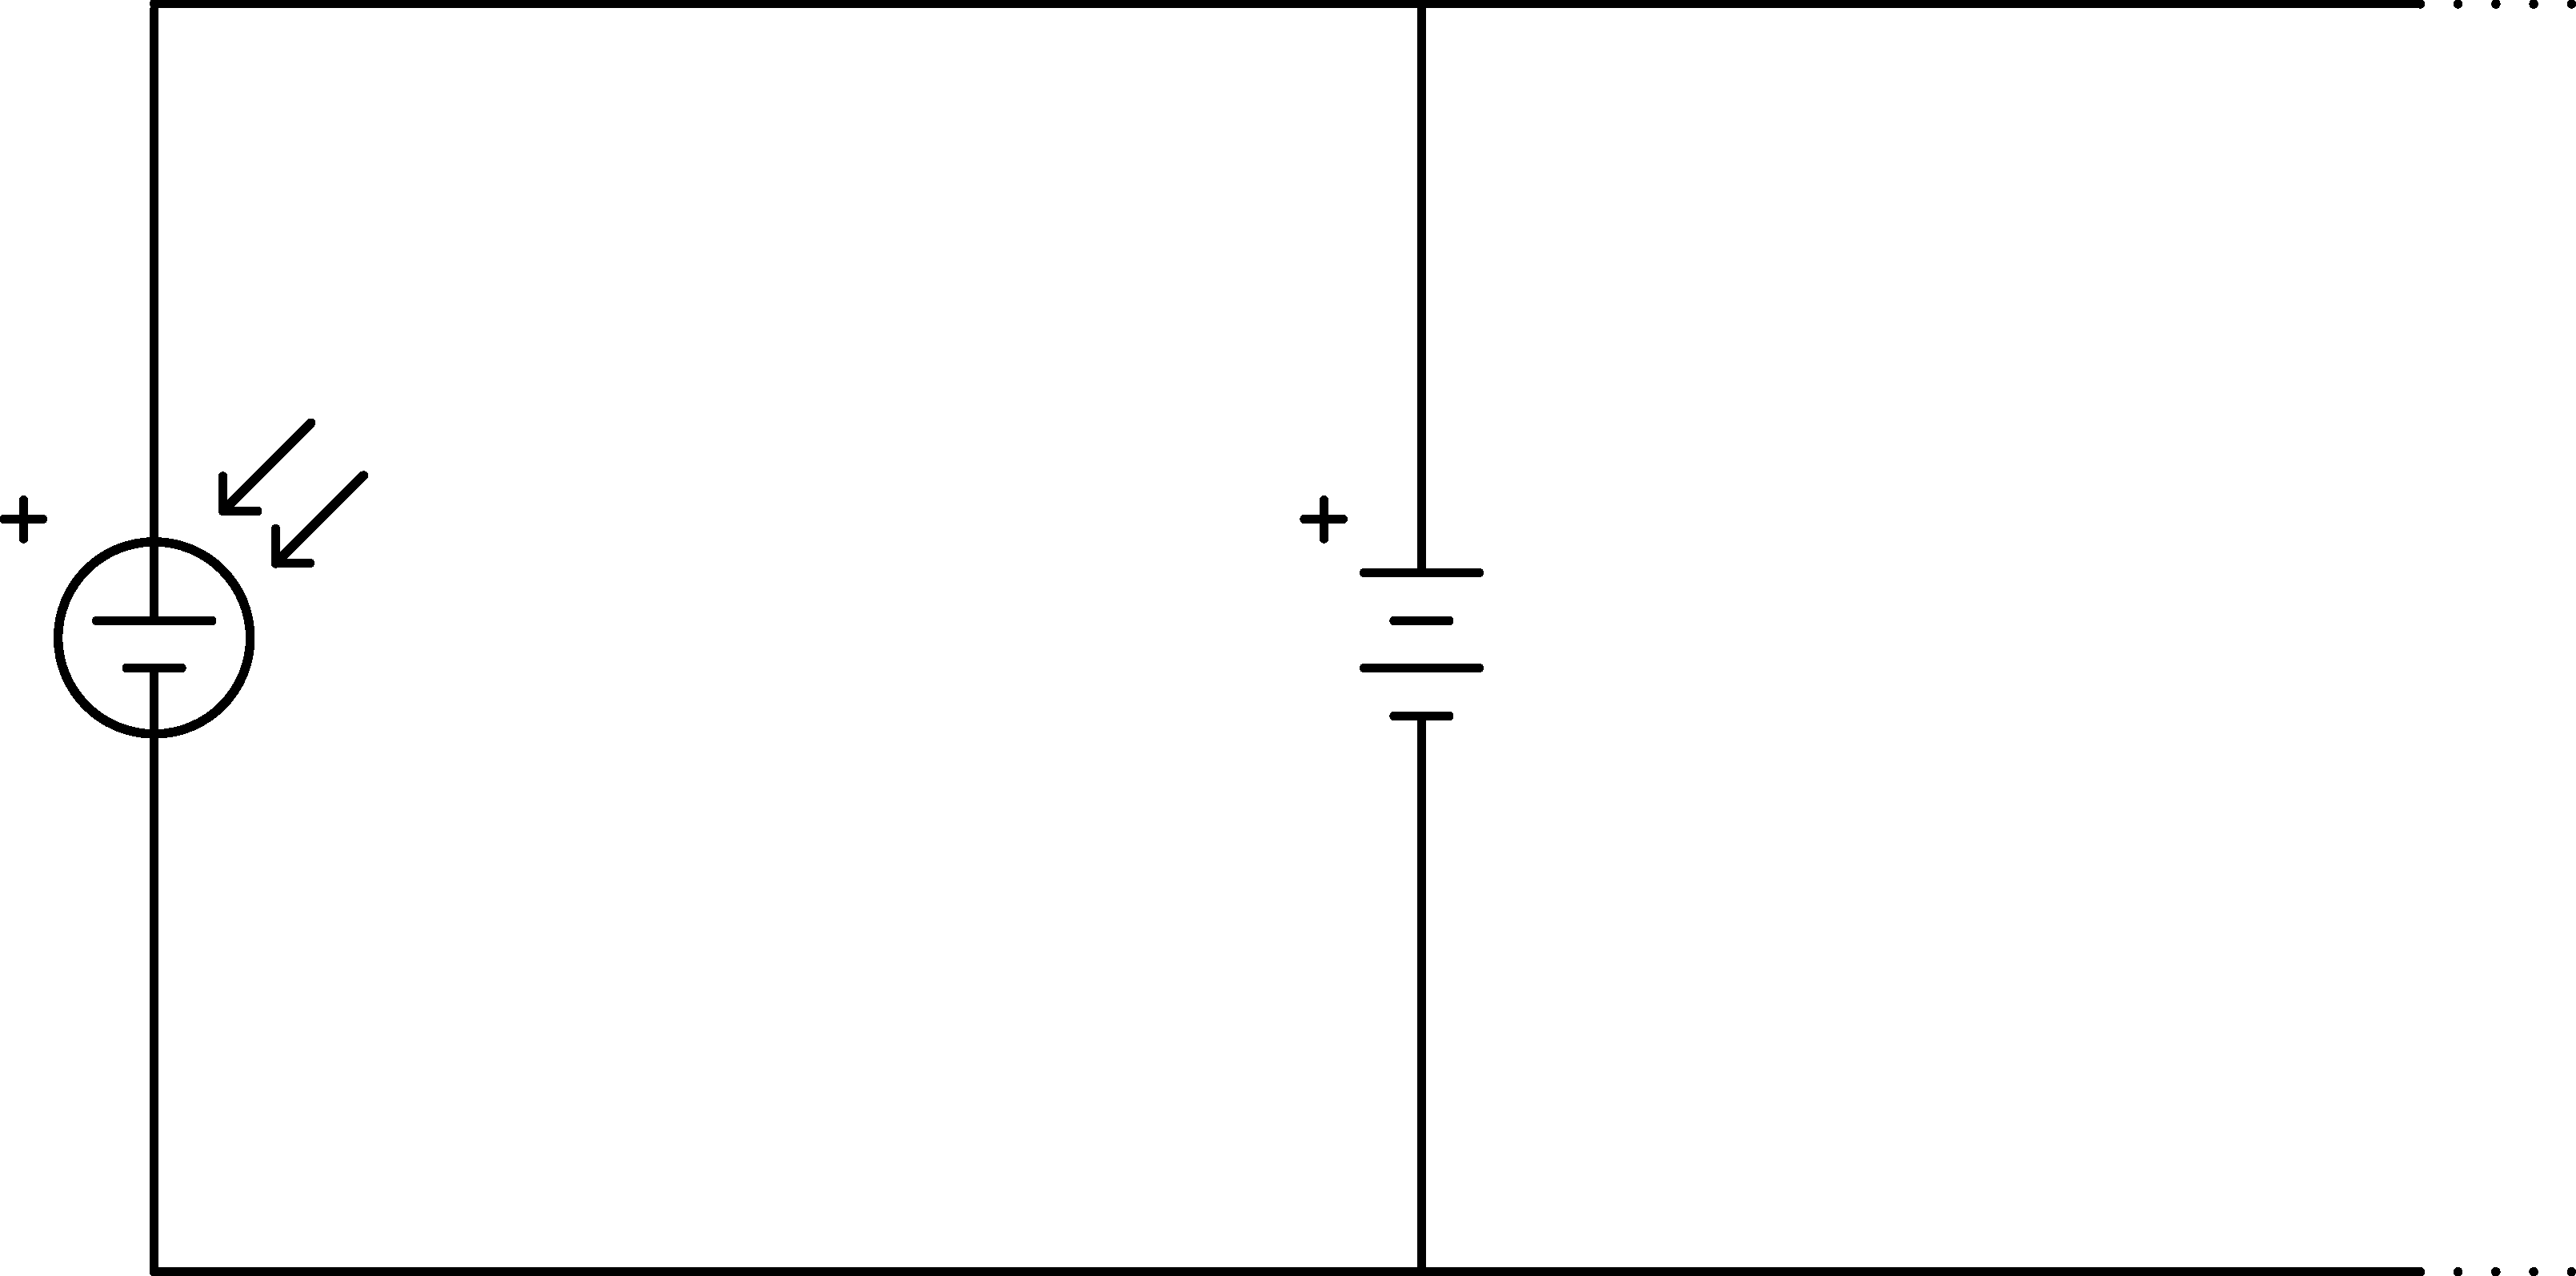
\includegraphics[width=0.75\linewidth]{versorgung_besipiel.pdf}
        \caption{Vereinfachte Darstellung der Stromversorgung}
    \end{figure}
    Dabei sind Steuer- und Regelelemente die das Speichermedium vor
    Schäden durch zu ofte Entladung schützen würden, sowie Filterelemente
    zur filterung Stromschwankungen ausgelassen.